\setchapterimage{fig_00.jpg}
\chapter*{TP 5 \\ 
Création d'un chemin auto-évitant -- \ifprof Corrigé \else Sujet \fi}
\addcontentsline{toc}{section}{TP 5 : 
Création d'un chemin auto-évitant -- \ifprof Corrigé \else Sujet \fi}

\iflivret \stepcounter{cptApplication} \else
\ifprof  \stepcounter{cptApplication} \else \fi
\fi

\setcounter{question}{0}
\marginnote{\url{https://doi.org/10.1098/rspa.2018.0549}}
Une marche auto-évitante est un processus au cours duquel un point décrit un chemin auto-évitant, c’est-à-dire qui ne se recoupe jamais lui-même. 

Dans ce sujet, on appellera chemin auto-évitant (CAE) de longueur $n$ tout ensemble de $n+1$ points $P_i = \left(x_i,y_i\right)\in \mathbb{Z}^2$ pour $0 \leq i \leq n$ tels que :
\begin{itemize}[label=$\blacktriangleright$]
\item $\forall i$, $||\vect{P_i P_{i + 1}}|| = 1$;
\item $\forall (i,j)$, $i\neq j \Rightarrow P_i \neq P_j$.
\end{itemize}



Chaque point du chemin sera représenté par une liste à deux éléments entiers précisant les deux coordonnées
(par exemple $P_i = \left(5, -4\right)$ est représenté par la liste \lstinline{[5,-4]}). Le chemin lui-même est constitué de la liste des points, dans l’ordre dans lequel ils sont atteints. Les codes Python produits dans cette partie devront manipuler exclusivement des coordonnées entières.
La figure \ref{02_CAE_fig_01} donne une représentation graphique de CAE de longueur 30 à partir de \lstinline{[0, 0]}.

\begin{marginfigure}
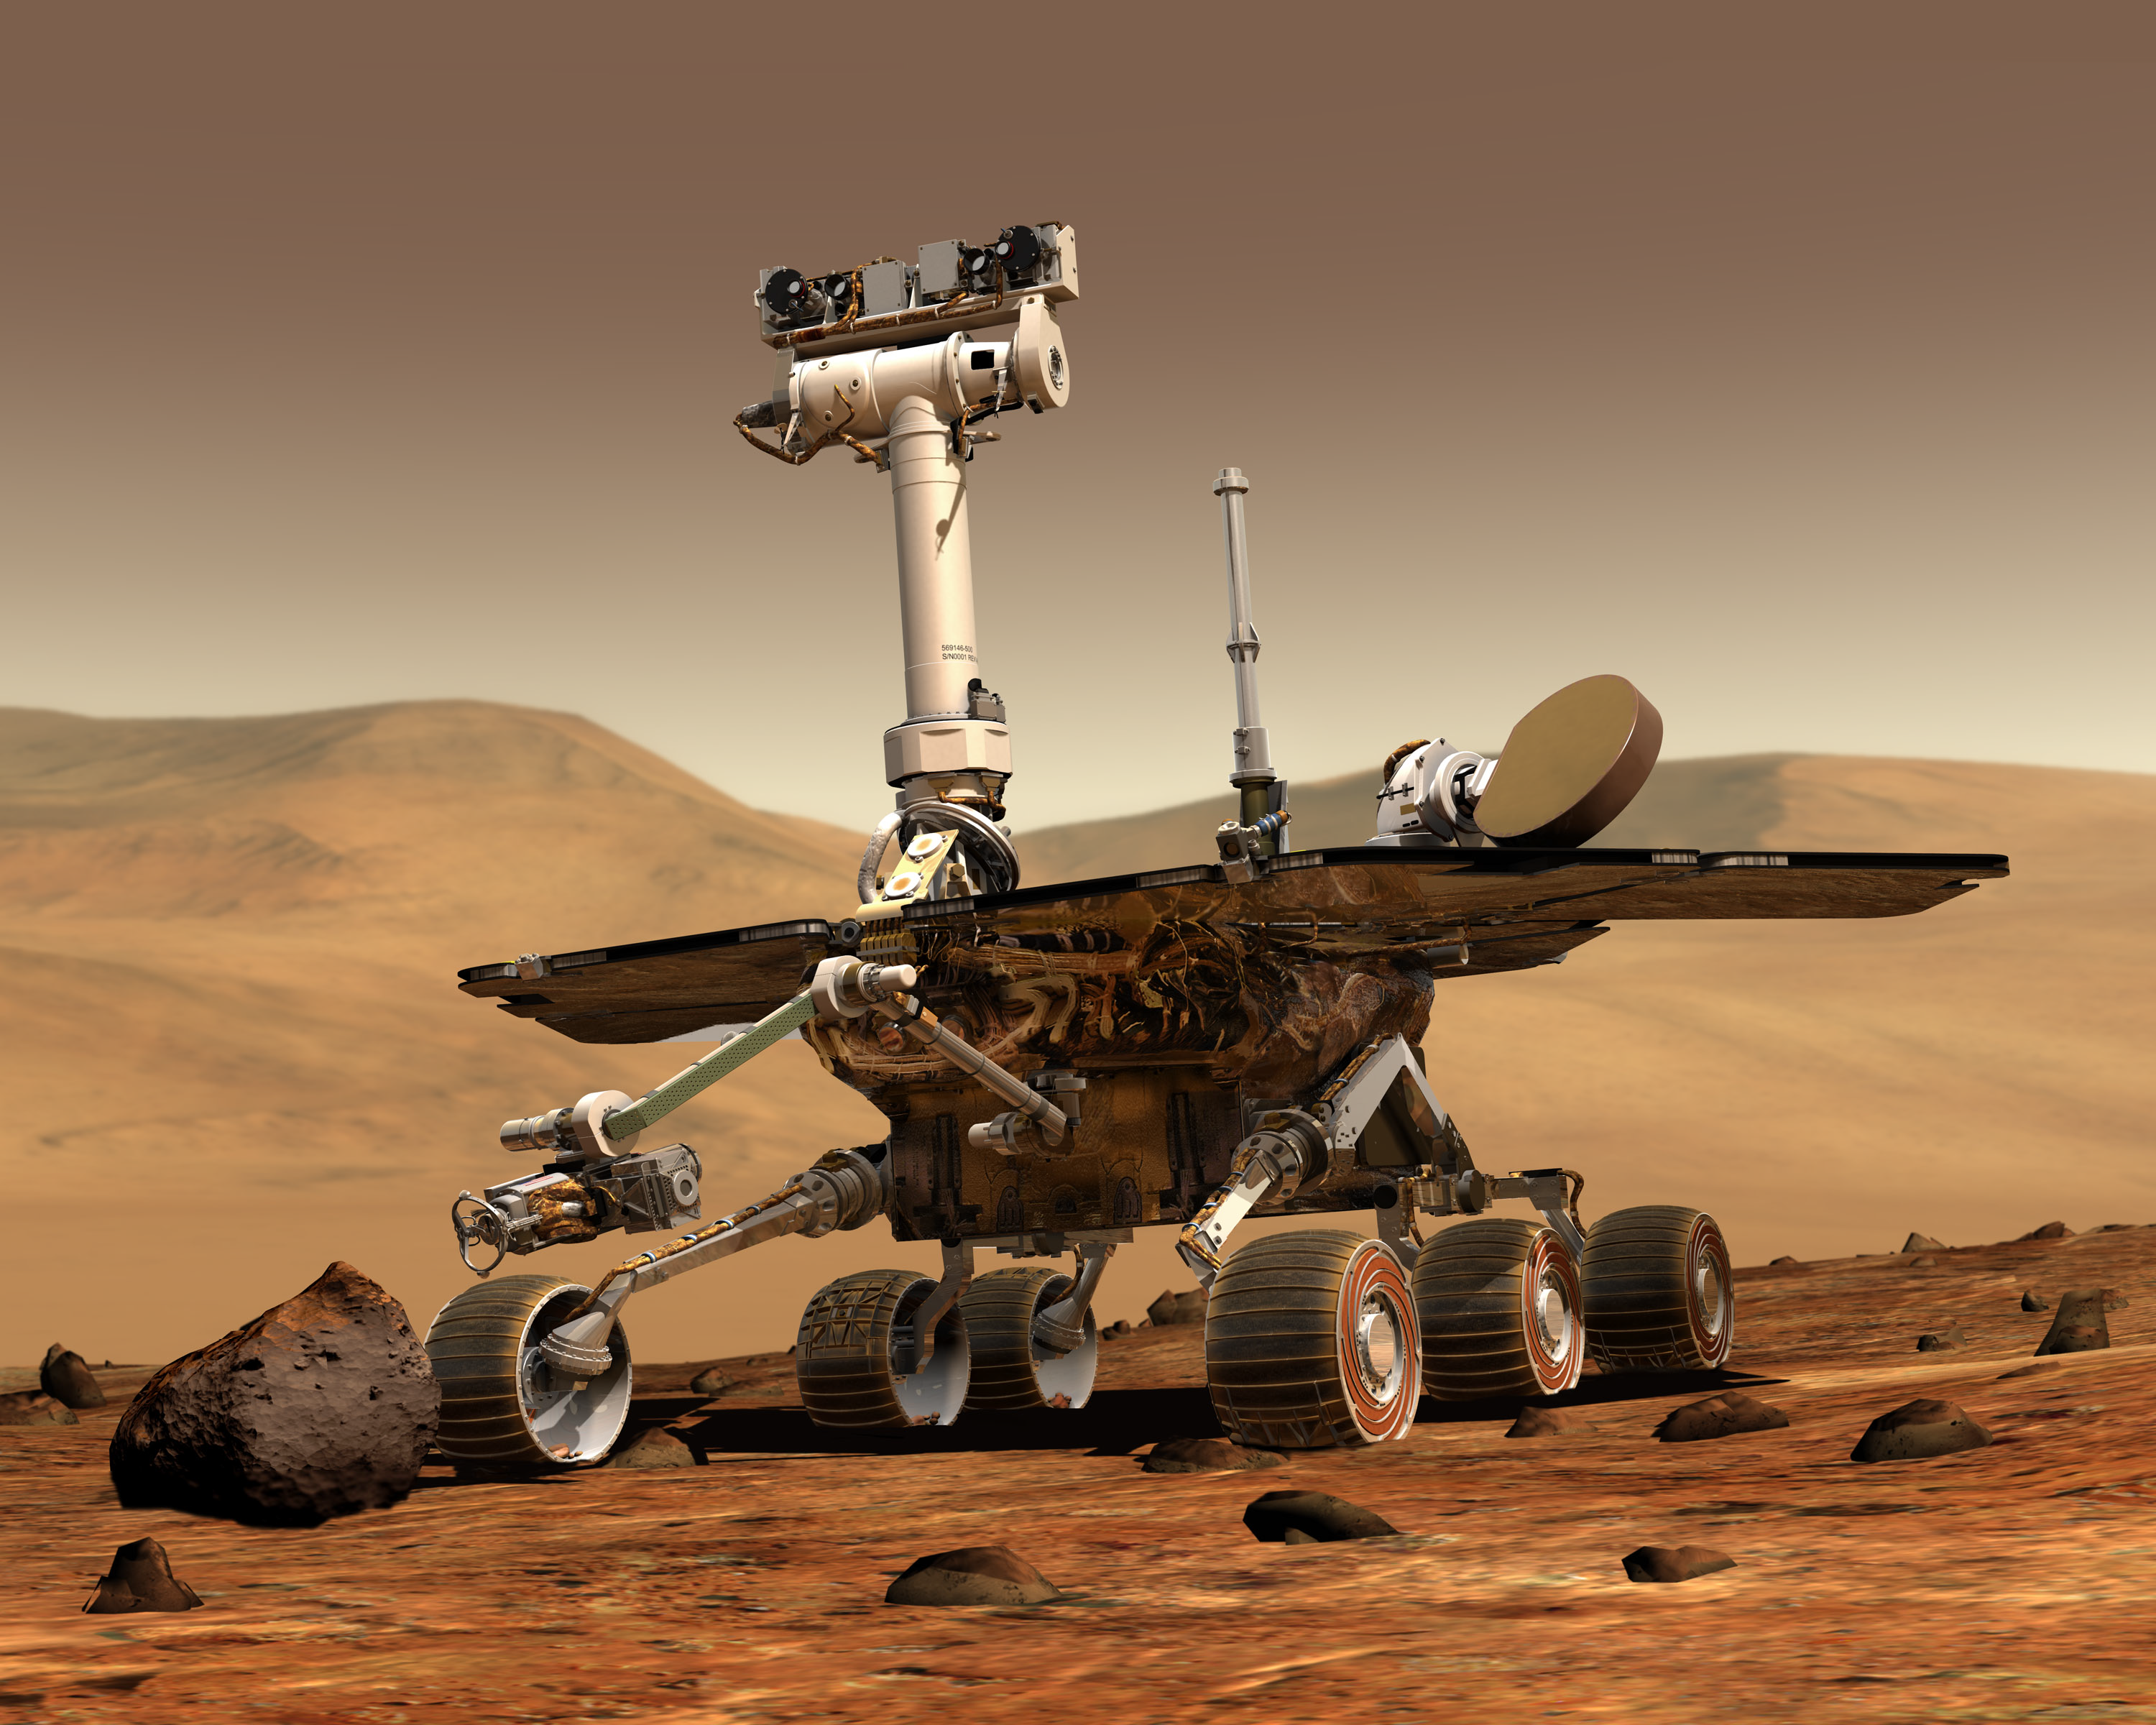
\includegraphics[width=\linewidth]{fig_01}
\caption{CAE de longueur 30\label{02_CAE_fig_01}}
\end{marginfigure}

\subsection*{Préambule - Tracé d'un chemin} 

On cherche d'abord à afficher un chemin quelquonque. 

Le module \lstinline{matplotlib} permet de réaliser des tracés. 


\begin{lstlisting}
# Import (et renommage) de la bibliothèque 
import matplotlib.pyplot as plt		# À écrire en tout début de fichier

les_x = [0,1,1,2]			# Liste des abscisses
les_y = [0,0,1,1]			# Liste des ordonnées

plt.plot(les_x,les_y,'-or')	# On affiche le tracé en rouge (r). Les points 
						# sont marqués par un cercle (o) 
						# et reliés par un trait (-). 

plt.grid()
plt.axis('equal')
plt.show() 						# Affiche la courbe

\end{lstlisting}


On appelle \lstinline{chemin} une liste de points, par exemple \lstinline{[[0,0],[1,0],[1,1],[2,1]]}.

\question{Après avoir importé les bibliothèques nécessaires, implémenter la fonction  \lstinline{plot_chemin(chemin:[[int]]) -> None} qui trace le chemin \lstinline{chemin}. Il faudra, à l'intérieur de cette fonction, créer les listes \lstinline{les_x} et \lstinline{les_y} des abscisses et des ordonnées de chacun des points .}



\begin{test}
\lstinline{plot_chemin([[0,0],[1,0],[1,1],[2,1]])} doit afficher la figure \ref{02_CAE_fig_03}.
\end{test}


\begin{marginfigure}
\includegraphics[width=\linewidth]{fig_03}
\caption{Affichage d'un chemin \label{02_CAE_fig_03}}
\end{marginfigure}





\subsection*{Chemin naïf} 


On s’intéresse dans un premier temps à une méthode naïve pour générer un chemin auto-évitant de longueur
$n$ sur une grille carrée. La méthode adoptée est une approche gloutonne :
\begin{enumerate}
\item le premier point est choisi à l’origine : $P_0 = \left(0, 0\right)$.
\item en chaque position atteinte par le chemin, on recense les positions voisines accessibles pour le pas
suivant et on en sélectionne une au hasard. En l’absence de positions accessibles l’algorithme échoue.
\item on itère l’étape 2 jusqu’à ce que le chemin possède la longueur désirée ou échoue.
\end{enumerate}





\question{Implémenter la fonction \lstinline{positions_voisines(p:[int]) -> [[int]]} qui construit la liste des positions voisines possibles à partir du point \lstinline{p}.}

\begin{test}
\lstinline{positions_voisines([0,0])} doit renvoyer \lstinline{[[0,1],[1,0],[0,-1],[-1,0]]}.
\end{test}


%L’expression booléenne \lstinline{v is None} indique si la valeur de \lstinline{v} est cette valeur spéciale.



\question{Implémenter la fonction \lstinline{positions_possibles(p:[int], chemin:[[int]]) -> [[int]]} qui construit la liste des positions suivantes possibles à partir du point \lstinline{p}. La liste \lstinline{chemin} contient les points déjà atteints.}

\begin{test}
\lstinline{positions_possibles([0,0],[])} doit renvoyer \lstinline{[[0, 1], [1, 0], [0, -1], [-1, 0]]}.

\lstinline{positions_possibles([0,1],[[0,0]])} doit renvoyer \lstinline{[[0, 2], [1, 1], [-1, 1]]}.
\end{test}




\question[Sur feuille]{Mettre en évidence graphiquement un exemple de CAE le plus court possible pour lequel, à une
étape donnée, la fonction \lstinline{positions_possibles} va renvoyer une liste vide. En prenant en compte les symétries, combien de tels chemins distincts existent pour cette longueur minimale ?}


Le module \lstinline{random} fournit la fonction \lstinline{randrange(a, b)} qui renvoie un entier compris entre \lstinline{a} et \lstinline{b-1} inclus, ainsi que la fonction \lstinline{choice(L)} qui renvoie l’un des éléments de la liste \lstinline{L}, dans les deux cas choisis aléatoirement avec une probabilité uniforme.

\begin{lstlisting}
# Import de la bibliothèque (et renommage en rd)
import random as rd 			# À écrire en tout début de fichier

print(rd.randrange(1,5))		# À utiliser où on veut dans le fichier
        						# Affiche aléatoirement 1, 2, 3 ou 4
L = [1,2,3]
rd.choice(L)				# Renvoie aléatoirement 1, 2, ou 3

\end{lstlisting}

%L’expression \lstinline{x in L} est une expression booléenne qui vaut \lstinline{True} si \lstinline{x} est l’un des éléments de \lstinline{L} et \lstinline{False} dans le cas contraire. On supposera que la méthode employée pour évaluer cette expression sur une liste est une recherche séquentielle.

%La valeur spéciale \lstinline{None} est utilisée en Python pour représenter une valeur invalide, inconnue ou indéfinie.

\question{Implémenter la fonction \lstinline{genere_chemin_naif(n:int) -> [[int]]} qui construit la liste des points représentant le
chemin auto-évitant de longueur \lstinline{n} en partant de l'origine $(0,0)$ et renvoie le résultat, ou bien renvoie la valeur spéciale \lstinline{[[]]} si à une
étape \lstinline{positions_possibles} renvoie une liste vide.}

\begin{test}
Tracer un chemin de longueur 20. Tracer un chemin de longueur 140. Que constatez-vous ?  
\end{test}


%\question{Évaluer avec soin la complexité temporelle asymptotique dans le pire des cas de la fonction \lstinline{genere_chemin_naif(n)} en fonction de \lstinline{n}, en supposant que la fonction ne renvoie pas \lstinline{None}.}
On souhaite connaître la probabilité de pouvoir obtenir un chemin autoévitant de taille $n$. 
Pour cela, pour des longueurs de chemin comprises entre 0 et 350, on peut calculer le taux de chemins réalisables.  


\begin{marginfigure}
\includegraphics[width=\linewidth]{fig_04}
\caption{Probabilité de pouvoir réaliser un CAE \label{02_CAE_fig_04}}
\end{marginfigure}



\question{En testant la possibilté de réaliser 1000 chemins pour chacune des longueurs comprises entre 1 et 350, tracer la probabilité qu'un chemin échoue en fonction de sa longueur (voir figure \ref{02_CAE_fig_04}).}


\question{Décrire ce que représente ce graphique et interpréter sa signification pour la méthode naïve.}

\subsection*{Methode du pivot}
Afin d’éviter les inconvénients de la méthode précédente, on s’intéresse à une solution différente nommée
méthode du pivot, proposée par Moti Lal en 1969. Son principe est le suivant :
\begin{enumerate}
\item on part d’un chemin auto-évitant arbitraire de longueur $n$. Ici, on choisira une initialisation très simple;
le chemin droit \lstinline{[[0, 0], [1, 0], [2, 0], ..., [n, 0]]};
\item on sélectionne au hasard un point, nommé pivot, entre le second et l’avant-dernier point du chemin,
et un angle aléatoire de rotation parmi $\pi$, $\dfrac{\pi}{2}$, $-\dfrac{\pi}{2}$;
\item on laisse les points avant le pivot inchangés et on fait subir à l’ensemble des points situés strictement
après le pivot une rotation ayant pour centre le pivot et pour angle, l’angle choisi à l’étape 2 ci-dessus;
\item si le chemin ainsi obtenu est auto-évitant, on le garde. Sinon, on reprend à l’étape 2 la sélection d’un
pivot et d’un angle, jusqu’à en trouver une paire qui convienne;
\item on répète les étapes 2 à 4 un certain nombre de fois. Le choix du nombre minimal de rotations à
effectuer pour obtenir un chemin non corrélé au chemin initial est laissé de côté dans ce sujet.
\end{enumerate}
Cette méthode permet de générer de manière efficace des marches auto-évitantes de plusieurs milliers de
points, comme la marche de longueur 2000 de la figure \ref{02_CAE_fig_02}.

\begin{marginfigure}
\includegraphics[width=\linewidth]{fig_02}
\caption{Marche de longueur 2000\label{02_CAE_fig_02}}
\end{marginfigure}

Dans cet algorithme, une étape importante est la vérification qu’un chemin donné est auto-évitant. Pour
vérifier cela on pourrait bien sûr s’y prendre comme dans la fonction \lstinline{positions_possibles}, mais on adopte une méthode différente avec une fonction \lstinline{est_CAE(chemin)} qui trie les points du chemin puis met à profit ce tri pour vérifier efficacement que le chemin est auto-évitant.

On utilise pour cela la fonction \lstinline{sorted} qui renvoie une nouvelle liste triée par ordre croissant. Elle fonctionne
sur tout type d’éléments disposant d’une relation d’ordre, y compris des listes pour lesquelles l’ordre lexicographique (ordre du premier élément, en cas d’égalité du second, etc.) est appliqué. %On suppose de plus que la complexité temporelle asymptotique dans le pire des cas de cette fonction est la meilleure possible.

%\question{Rappeler, sans la justifier, la complexité temporelle asymptotique dans le pire des cas attendue de sorted en fonction de la longueur de la liste à trier. Donner le nom d’un algorithme possible pour son implémentation.}

%En utilisant le canevas fourni en annexe et en ajoutant les import nécessaires :
\marginnote{
On rappelle qu'un chemin de longueur $n$ est auto-évitant si pour $0 \leq i \leq n$ :
\begin{itemize}[label=$\blacktriangleright$]
\item $\forall i$, $||\vect{P_i P_{i + 1}}|| = 1$;
\item $\forall (i,j)$, $i\neq j \Rightarrow P_i \neq P_j$.
\end{itemize}
}
\question{Implémenter la fonction \lstinline{est_CAE(chemin:[[int]]) -> bool} qui vérifie si un chemin est auto-évitant en se basant sur \lstinline{sorted}.}% Elle devra ne pas être de complexité temporelle asymptotique dans le pire des cas supérieure à la fonction \lstinline{sorted} : vous prouverez ce dernier point.}

\question{Implémenter la fonction \lstinline{rot(p:[int], q:[int], a:int) -> [int]} qui renvoie le point image du point \lstinline{q} par la rotation de centre \lstinline{p} et d’angle défini par la valeur de \lstinline{a} : \lstinline{0} pour $\pi$, \lstinline{1} pour $\dfrac{\pi}{2}$, \lstinline{2} pour $-\dfrac{\pi}{2}$.}


\question{Implémenter la fonction \lstinline{rotation(chemin:[[int]], i_piv:int, a:int) -> [[int]]} qui renvoie un nouveau chemin identique à \lstinline{chemin} jusqu’au pivot d’indice \lstinline{i_piv}, et ayant subi une rotation de \lstinline{a} autour du pivot (même codage que la fonction précédente) sur la partie strictement après le pivot.}

\question{Implémenter la fonction \lstinline{genere_chemin_pivot(n:int, n_rot:int) -> [[int]]} permettant de générer un chemin autoévitant de longueur \lstinline{n} en appliquant \lstinline{n_rot} rotations. L’application d’une rotation peut nécessiter plusieurs tentatives.}

%\question{On considère un pivot, son point précédent et son point suivant. Quel est l’impact prévisible sur les rotations admissibles ? Suggérer un moyen de prendre en compte cette propriété pour améliorer l’algorithme.}
